\epi{\lstinline{fmt.Printf("\%p", i)}}{Printing the address of a pointer in Go.}
\noindent{}
You may have wished otherwise, but Go has pointers.
There is however no pointer arithmetic, so they act more like
references than pointers that you may know from C. Pointers as
they are still called in Go are useful.
Remember when you call a function in Go the variables you pass are
pass-by-value. So, for efficiency and the possibility to modify a
passed value \emph{in} the function we have pointers.

Just like in C you declare a pointer by prefixing the type with an `*`:
\lstinline{var p *int}. Now \var{p} is a pointer to an integer value.
All newly declared variables are assigned their zero value and pointer
are no difference. A newly declared, or just a pointer that points to
nothing has a \first{nil}-value. In other languages this is often called
a NULL pointer in Go it is just \var{nil}. To make 
a pointer point to something you can use the address-of operator
(\func{\&}), which we do on line 5:
\begin{lstlisting}[caption=Make use of a pointer,numbers=right,label=src:pointers]
var p *int	    
fmt.Printf("%v", p) |\coderemark{Prints \var{nil}}|

var i int	    |\coderemark{Declare integer variable \var{i}}|
p = &i		    |\coderemark{Make \var{p} point to \var{i}}|

fmt.Printf("%v", p) |\coderemark{Prints something like \var{0x7ff96b81c000a}}|
\end{lstlisting}

More general: \var{*X} is a pointer to an \type{X}; \var{[3]X} is an
array of three \type{X}'s. The
types are therefore really easy to read just read out the names of the
type modifiers: \type{[]} declares something called an array slice; "*"
declares a pointer; \type{[size]} declares an array. So
\type{[]*[3]*int} is an array slice of pointers to arrays of three
pointers to \type{int}s

\section{Allocation}
Go has garbage collection, meaning that you don't have to worry about
memory allocation and deallocation. Of course almost every language
since 1980 has this, but it is nice to see garbage collection in a
C-like language. The following sections show how to handle allocation
in Go. There is somewhat an artifical distinction between
\first{\func{new()}} and \first{\func{make()}}. Details follow.

\subsection{Nil value}
A reference to nothing is represented in Go as \lstinline{nil}. This is
different than a zero value. \todo{nil only for references?}

\begin{lstlisting}
var *a int
a = nil
fmt.Printf("%v\n", a);
\end{lstlisting}
Prints \lstinline{nil}.

\subsection{Conversions}
\label{sec:conversions}
Sometimes you want to convert a type to another type. In C this is known
as casting a value to another type. This is also possible in Go, but
there are some rules.\todo{there are more rules, but we're trying to
keep it simple...}
You can convert:
\begin{itemize}
\item{
From a \lstinline{string} to a slice of \lstinline{byte}s.
\begin{lstlisting}
mystring = "hello this is string"
byteslice =  []byte(mystring)
\end{lstlisting}
}
\item{
From a slice of \lstinline{byte}s to a \lstinline{string}.
\begin{lstlisting}
The other way around
\end{lstlisting}
}
\end{itemize}

\subsection{Allocation with \func{new()}}
Go has two allocation primitives, \func{new()} and \func{make()}. They do different
things and apply to different types, which can be confusing, but the
rules are simple. Let's talk about \func{new()} first. It's a built-in function
essentially the same as its namesakes in other languages: \func{new(T)}
allocates zeroed storage for a new item of type \type{T} and returns its
address, a value of type \type{*T}. In Go terminology, it returns a pointer to
a newly allocated zero value of type \type{T}.

Since the memory returned by \func{new()} is zeroed, it's helpful to arrange
that the zeroed object can be used without further initialization. This
means a user of the data structure can create one with \func{new()} and get
right to work. For example, the documentation for \type{bytes.Buffer} states
that "the zero value for Buffer is an empty buffer ready to use."
Similarly, \func{sync.Mutex} does not have an explicit constructor or Init
method. Instead, the zero value for a \func{sync.Mutex} is defined to be an
unlocked mutex.

The zero-value-is-useful property works transitively. Consider this type
declaration.

\begin{lstlisting}
type SyncedBuffer struct {
    lock    sync.Mutex
    buffer  bytes.Buffer
}
\end{lstlisting}
Values of type \type{SyncedBuffer} are also ready to use immediately upon
allocation or just declaration. In this snippet, both \var{p} and
\var{v} will work
correctly without further arrangement.
\begin{lstlisting}
p := new(SyncedBuffer)  // type *SyncedBuffer
var v SyncedBuffer      // type  SyncedBuffer
\end{lstlisting}

\subsection{Allocation with \func{make()}}
Back to allocation. The built-in function \func{make(T, args)} serves a purpose
different from \func{new(T)}. It creates slices, maps, and channels only, and
it returns an initialized (not zero) value of type T, not *T. The reason
for the distinction is that these three types are, under the covers,
references to data structures that must be initialized before use. A
slice, for example, is a three-item descriptor containing a pointer to
the data (inside an array), the length, and the capacity; until those
items are initialized, the slice is nil. For slices, maps, and channels,
make initializes the internal data structure and prepares the value for
use. For instance,
\lstinline{make([]int, 10, 100)}
allocates an array of 100 ints and then creates a slice structure with
length 10 and a capacity of 100 pointing at the first 10 elements of the
array. (When making a slice, the capacity can be omitted; see the
section on slices for more information.) In contrast, new([]int) returns
a pointer to a newly allocated, zeroed slice structure, that is, a
pointer to a nil slice value.

These examples illustrate the difference between new() and make().
\begin{lstlisting}
var p *[]int = new([]int)       // allocates slice structure; *p == nil; rarely useful
var v  []int = make([]int, 100) // v now refers to a new array of 100 ints

// Unnecessarily complex:
var p *[]int = new([]int)
*p = make([]int, 100, 100)

// Idiomatic:
v := make([]int, 100)
\end{lstlisting}
Remember that make() applies only to maps, slices and channels and does
not return a pointer. To obtain an explicit pointer allocate with new().

\subsection{Constructors and composite literals}
Sometimes the zero value isn't good enough and an initializing
constructor is necessary, as in this example derived from package
\package{os}.
\begin{lstlisting}
func NewFile(fd int, name string) *File {
    if fd < 0 {
        return nil
    }
    f := new(File)
    f.fd = fd
    f.name = name
    f.dirinfo = nil
    f.nepipe = 0
    return f
}
\end{lstlisting}
There's a lot of boiler plate in there. We can simplify it using a
composite literal, which is an expression that creates a new instance
each time it is evaluated.

\begin{lstlisting}
func NewFile(fd int, name string) *File {
    if fd < 0 {
        return nil
    }
    f := File{fd, name, nil, 0}
    return &f
}
\end{lstlisting}
Note that it's perfectly OK to return the address of a local variable;
the storage associated with the variable survives after the function
returns. In fact, taking the address of a composite literal allocates a
fresh instance each time it is evaluated, so we can combine these last
two lines.

\begin{lstlisting}
return &File{fd, name, nil, 0}
\end{lstlisting}
The fields of a composite literal are laid out in order and must all be
present. However, by labeling the elements explicitly as field:value
pbairs, the initializers can appear in any order, with the missing ones
left as their respective zero values. Thus we could say

\begin{lstlisting}
return &File{fd: fd, name: name}
\end{lstlisting}
As a limiting case, if a composite literal contains no fields at all, it
creates a zero value for the type. The expressions
\lstinline{new(File)} and 
\lstinline|&File{]| are equivalent.

Composite literals can also be created for arrays, slices, and maps,
with the field labels being indices or map keys as appropriate. In these
examples, the initializations work regardless of the values of Enone,
Eio, and Einval, as long as they are distinct.
\begin{lstlisting}
a := [...]string   {Enone: "no error", Eio: "Eio", Einval: "invalid argument"}
s := []string      {Enone: "no error", Eio: "Eio", Einval: "invalid argument"}
m := map[int]string{Enone: "no error", Eio: "Eio", Einval: "invalid argument"}
\end{lstlisting}


\section{Defining your own}
\label{sec:defining your own}
Ofcourse Go allows you to define new types, it does this in (almost) the
same way as in C, with the \key{struct} keyword.

An empty struct is created with \lstinline|var empty struct {}|{}.
A more real-life example would be when we want record seomebody's name
and age in a single ... TODO. We could do

\lstinputlisting[label=src:struct,caption=Structures]{src/struct.go}

Apropos, the output of \lstinline{fmt.Printf("\%v\n", a)} is 
\begin{display}
{Pete, 42}
\end{display}
How nice is that, Go knows how to print your structure! If you
only want to print a one, or a few, field of the structure you'll
need to use \verb|<field name>|. To only print the name:
\begin{lstlisting}
fmt.Printf("%s", a.name) |\coderemark{\%s formats a string}|
\end{lstlisting}

Defining a new type:

\begin{lstlisting}
type T struct {
    name string // name of the object
    value int // its value
}
\end{lstlisting}

Or alias a build in one.
Methods on types, and methods on build in type -- can not do that,
just create a new type.

\section{Interfaces}
%%\epi{I have this phobia about having my body penetrated surgically. You
%%know what I  mean?}{\textit{eXistenZ}\\\textsc{Ted Pikul}}
One of the interesting aspects of the Go language is \first{interface objects}.
\gomarginpar{The following text is copied (and slightly shortend) from \cite{go_interfaces} which is
written by Ian Lance Taylor - one of the original authors of Go.}
In Go, the word interface is overloaded to mean several different
things. Every type has an \first{interface}, which is the set of methods defined for
that type. This bit of code defines a struct type \type{S} with one field, and
defines two methods for \type{S}.
\begin{lstlisting}[caption=Defining a struct and methods,label=src:interface object]
type S struct { i int }
func (p *S) Get() int { return p.i }
func (p *S) Put(v int) { p.i = v }
\end{lstlisting}
You can also define an \first{interface type}, which is simply a set of methods.
This defines an interface \type{I} with two methods:
\begin{lstlisting}
type I interface {
  Get() int;
  Put(int);
}
\end{lstlisting}
\type{S} is a valid implementation for \type{I}, because it defines the two 
methods which \type{I} requires. Note that this is true even though there is 
no explicit declaration that \type{S} implements \type{I}. A Go program can use 
this fact via yet another meaning of interface, which is an \first{interface value}:

\begin{lstlisting}
func f(p I) { fmt.Println(p.Get()); p.Put(1) }
\end{lstlisting}
Here the variable \var{p} holds a value of interface type. Because
\type{S}
implements \type{I}, we can call \func{f} passing in a pointer to a value of type
\type{S}:

\begin{lstlisting}
var s S; f(&s)
\end{lstlisting}
The reason we need to take the address of \type{S}, rather than a value of type
\type{S}, is because we defined the methods on \type{S} to operate on
pointers, see the code above in listing \ref{src:interface objects}.
This
is not a requirement --- we could have defined the methods to take
values --- but then the \func{Put} method would not work as expected.

The fact that you do not need to declare whether a type implements an
interface means that Go implements a form of \first{duck typing}. This is not
pure duck typing, because when possible the Go compiler will statically
check whether the type implements the interface. However, Go does have a
purely dynamic aspect, in that you can convert from one interface type
to another. In the general case, that conversion is checked at runtime.
If the conversion is invalid --- if the type of the value stored in the
existing interface value does not satisfy the interface to which it is
being converted --- the program will fail with a runtime error.

Interfaces in Go are similar to ideas in several other programming languages:
pure abstract virtual base classes in C++, typeclasses in Haskell or duck typing
in Python. However there is no other language which combines
interface values, static type checking, dynamic runtime conversion, and no
requirement for explicitly declaring that a type satisfies an interface. The
result in Go is powerful, flexible, efficient, and easy to write.

\subsection{Empty interface}
For example, since every type satisfies the empty interface:
\type{interface \{\}}. We can create a generic function which 
has an empty interface as its argument:
\begin{lstlisting}[caption=A function with a empty interface
argument,label=src:interface empty]
func g(any interface{}) int { return any.(I).Get() }
\end{lstlisting}
The \lstinline{return any.(I).Get()} is the tricky bit in this function.
The value \var{any} has type \type{interface{}}, meaning no guarantee
of any methods at all: it could contain any type. The \lstinline{.(I)}
is a \first{type switch} which converts \var{any} to an interface of
type \type{I}. If we have that type we can invoke the \func{Get()}
function.
So if we create a new variable of the type \type{*S}, we can just
call \func{g()}, because \type{*S} also implements the empty interface.
\begin{lstlisting}
s = new(S)
fmt.Println(g(s));
\end{lstlisting}
The call to \func{g} will work fine and will print 0. If we however
invoke \func{g()} with a value that does not implement \type{I} we have
a problem:
\begin{lstlisting}[caption=Failing to implement an interface,label=src:interface fail]
i := 5		// make i a "lousy" int
fmt.Println(g(i))
\end{lstlisting}
This compiles OK, but when we run this we get slammed with:

\noindent\error{panic: interface conversion: int is not main.I: missing
method Get}

\noindent{}Which is completely true, the built-in type \type{int} does not
have a \func{Get()} function.

\subsection{Methods}
You can also define functions (or better called methods from now on) on
interfaces. In fact, any value, and type can have methods. 
You can make an integer type with its own methods. For example:
\begin{lstlisting}
type Foo int;

func (self Foo) Emit() {
  fmt.Printf("\%v", self);
}

type Emitter interface {
  Emit();
}
\end{lstlisting}

\section{Interface names}
By convention, one-method interfaces are named by the method name plus
the \emph{-er} suffix: Read\emph{er}, Writ\emph{er}, Formatt\emph{er} etc.

There are a number of such names and it's productive to honor them and
the function names they capture. Read, Write, Close, Flush, String and
so on have canonical signatures and meanings. To avoid confusion, don't
give your method one of those names unless it has the same signature and
meaning. Conversely, if your type implements a method with the same
meaning as a method on a well-known type, give it the same name and
signature; call your string-converter method String not ToString.
from \cite{effective_go}.


\section{Introspection}
A \key{switch} can also be used to discover the dynamic type of an interface
variable. Such a type switch\gomarginindex{\emph{type switch}}{type switch} uses
the syntax of a type assertion with the keyword type inside the
parentheses. If the switch declares a variable in the expression, the
variable will have the corresponding type in each clause.
\begin{lstlisting}[caption=Dynamically find out the type]
package main
type PersonAge struct { |\longremark{First we define two structures as a new type, %
\texttt{PersonAge};}|
	name string
	age  int
}

type PersonShoe struct { |\longremark{And \texttt{PersonShoe};}|
	name     string
	shoesize int
}

func main() {
	p1 := new(PersonAge)
	p2 := new(PersonShoe)
	WhichOne(p1)
	WhichOne(p2)
}

func WhichOne(x interface{}) { |\longremark{This function must accept \emph{both} %
types as valid input, so we use the empty Interface, which every type implements;}|
	switch t := x.(type) { |\longremark{The type switch: \texttt{(type)};}|
	case *PersonAge:	|\longremark{When allocated with \func{new} its a %
pointer. So we check for \type{*PersonAge}. If \func{WhichOne()} was %
called with a non pointer value, we should check for \type{PersonAge}.}|
		println("Age person")
	case *PersonShoe:
		println("Shoe person")
	}
}
\end{lstlisting}
\showremarks

The following is another example of performing a type switch, but this
time checking for more (built-in) types:
\begin{lstlisting}[caption=A more generic type switch]
switch t := interfaceValue.(type) { |\coderemark{The type switch}|
default:
    fmt.Printf("unexpected type %T", t)  // \%T prints type
case bool:
    fmt.Printf("boolean %t\n", t)
case int:
    fmt.Printf("integer %d\n", t)
case *bool:
    fmt.Printf("pointer to boolean %t\n", *t)
case *int:
    fmt.Printf("pointer to integer %d\n", *t)
}
\end{lstlisting}

\subsection{Introspection and reflection}
\label{subsec:introspection and reflection}
In the following example we want to look at the "tag" (here named
"namestr") defined in the
type definition of \type{Person}. We are using the
\package{reflect} package (there is no other way in Go). Keep in mind
that looking at a tag means going back the \emph{type} definition. So
use the \package{reflect} we need figure out the type of the variable
and then access the tag.

\begin{lstlisting}[caption=Introspection using reflection,label=src:introspection]
|\begin{tikzpicture}[overlay]
\draw [->,thick] (2.8,-6.00) node [left] %
{\longremark{We are dealing with a \type{PtrValue} and according %
to the documentation\footnote{\texttt{godoc reflect}}:%
\begin{quote} %
\texttt{\func{func} (v *PtrValue) Elem() Value}\\%
Elem returns the value that v points to. %
If v is a nil pointer, Elem returns a nil Value. %
\end{quote} %
we can use \func{Elem()} to get the type the pointer points to. %
In this case \type{*reflect.StructValue};}} %
to (2.8,-5.20);
%
\draw [->,thick] (3.8,-6.00) node [left] %
{\longremark{\func{Type()} returns \type{reflect.Type};}} %
to (3.8,-5.20);
\draw [->,thick] (5.4,-6.00) node [left] %
{\longremark{%
Again according to the documentation, we have:\\%
\begin{quote} %
\ldots which returns an object with interface %
type \type{Type}.  That contains a pointer to a struct of type %
\type{*StructType}, %
\type{*IntType}, etc. representing the details of the underlying type. %
A type switch or type assertion can reveal which. %
\end{quote} %
So we can access your specific type as a member of this struct. Which %
we do with \type{(*reflect.StructType)};}} %
to (5.4,-5.20);
%
\draw [->,thick] (6.8,-6.00) node [left] %
{\longremark{%
A \type{StructType} has a number of methods, one of which is %
\func{Field($n$)} which returns the $n^{th}$ field of a structure. %
The type of this return is a \type{StructField}; %
}} %
to (6.8,-5.20);
%
\draw [->,thick] (8.4,-6.00) node [left] %
{\longremark{We finally have the type we are after. Now we can use the %
methods defined for \type{*StructType}, like \func{Field(n)}, which %
returns the n$^{th}$ field of our struct as a \type{StructField};}} %
to (8.4,-5.20);
%
\draw [->,thick] (9.4,-6.00) node [left] %
{\longremark{The struct \type{StructField} has a \var{Tag} member which %
returns the tag-name as a string. So on the $0^{th}$ field we can %
unleash \func{.Tag} to access this name: \texttt{Field(0).Tag}. This %
\emph{finally} gives us \texttt{namestr}.}}%
to (9.4,-5.20);
\end{tikzpicture}|
type Person {
    name string "namestr"
    age  int
}

p1 := new(Person)   |\coderemark{\func{new} returns a pointer to Person}|
ShowTag(p1)	    |\coderemark{\func{ShowTag()} is now called with this pointer}|

func ShowTag(i interface{}) {
    switch t := reflect.NewValue(i).(type) { |\coderemark{Type assertion}|
    case *reflect.PtrValue:		     |\coderemark{\var{p1} is a pointer}|
	tag := t.Elem().Type().(||*reflect.StructType).Field(0).Tag
||
\end{lstlisting}

\showremarks

%% look at layout
To make the difference between looking a types and values more clear,
that a look at the following code:
\begin{lstlisting}[caption=Reflection and the type and value]
func show(i interface{}) {
    switch t := i.(type) {
      case *Person:
        r := reflect.NewValue(i) |\coderemark{Enter the world of reflection}|
	tag := |\longremark{Here we want to get the "tag", which means %
going for the type. Thus we need\newline\lstinline{Elem().Type().(*reflect.StructType)} to get to it;}|
	  r.(*reflect.PtrValue).Elem().Type().(*reflect.StructType).Field(0).tag
	nam := |\longremark{Now we want to get access to the %
\emph{value} of one of the members and we %
employ\newline\lstinline{Elem().(*reflect.StructValue)} to get to it. %
Now we have arrived at the structure. Then we go the the first field %
\lstinline{Field(0)}, tell \package{reflect} is a %
\var{*reflect.StringValue} and invoke the \lstinline{Get()} method on %
it. %
\begin{figure}[H] %
\hskip3\baselineskip\parbox{0.7\textwidth}{\caption[Pealing away the layers using reflection]{Pealing away the %
layers using reflection. %
Going from a \type{*Person} via \mbox{\type{*reflect.PtrValue}} using the %
methods described in \prog{godoc reflect} to get the %
actual \type{string} contained deep within.}} %
\label{fig:reflection} %
\begin{center} %
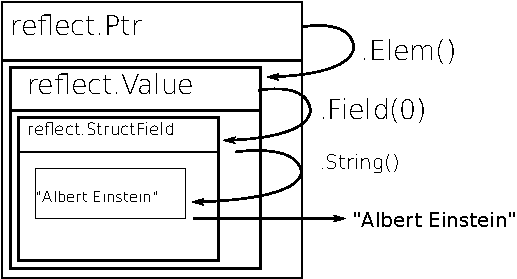
\includegraphics[scale=0.85]{fig/reflection.pdf} %
\end{center}\end{figure} %
Reflection works by pealing off layers once you have got your hands %
on a \type{Value} in the reflection world.
}|
	  r.(*reflect.PtrValue).Elem().(*reflect.StructValue).Field(0)\newline.(*reflect.StringValue).Get()
\end{lstlisting}
\showremarks




Setting a value works similarly as getting a value, but only works on
\emph{exported} members. Again some code:

\begin{minipage}{.5\textwidth}
\begin{lstlisting}[caption=Reflect with private member]
type Person struct {
 name string "namestr"
 age  int
}

func Set(i interface{}) {
 switch t := i.(type) {
 case *Person:
  r := reflect.NewValue(i)
  r.(*reflect.PtrValue).Elem().
    (*reflect.StructValue).
    FieldByName("name").
    (*reflect.StringValue).
    Set("Albert Einstein")
  }
}
\end{lstlisting}
\end{minipage}
\begin{minipage}{.5\textwidth}
\begin{lstlisting}[caption=Reflect with public member]
type Person struct {
 Name string "namestr" |\coderemark{}|
 age  int
}

func Set(i interface{}) {
 switch t := i.(type) {
 case *Person:
  r := reflect.NewValue(i)
  r.(*reflect.PtrValue).Elem().
   (*reflect.StructValue).
   FieldByName("Name"). |\coderemark{}|
   (*reflect.StringValue).
   Set("Albert Einstein")
  }
}
\end{lstlisting}
\end{minipage}
The code on the left compiles and runs, but when you run it, you are greeted with a
stack trace and a \emph{runtime} error:

\noindent\error{panic: cannot set value obtained via unexported struct
field}

\noindent{}The code on the right works OK and sets the member \var{Name}
to "Albert Einstein". Of course this only works when you call \func{Set()}
with a pointer argument.


\section{Exercises}
\begin{Exercise}[title={Interfaces and compilation},difficulty=6]
\Question
The code in listing \ref{src:interface fail} compiles OK --- as stated 
in the text. But when you run it you'll get a runtime error, so
something \emph{is} wrong. Why does the code compile cleanly then?
\end{Exercise}

\begin{Answer}
\Question
The code compiles because an integer type implements the empty interface
and that is the check that happens at compile time.

A proper way to fix this, is to test if such an empty interface can
be converted and if so, call the appropriate method. The Go code
that defines the function \func{g} in listing \ref{src:interface empty}
-- repeated here:
\begin{lstlisting}
func g(any interface{}) int { return any.(I).Get() }
\end{lstlisting}

\noindent{}Should be changed to become:
\begin{lstlisting}
func g(any interface{}) int {
    if v, ok := any.(I); ok {	// Check if any can be converted
	return v.Get()		// If so invoke Get()
    }
    return -1			// Just so we return anything
}
\end{lstlisting}
If \func{g()} is called now there are no run-time errors anymore. The
idiom used is called "comma ok" in Go.
\end{Answer}


\begin{Exercise}[title={指针},difficulty=6]
\label{ex:pointers}

\Question
假设定义了下面的结构:
\begin{lstlisting}
type Person struct {
    name string
    age	 int
}
\end{lstlisting}

下面两行之间的区别是什么?
\begin{lstlisting}
var p1 Person
p2 := new(Person)
\end{lstlisting}

\Question
下面两个内存分配的区别是什么?
\begin{lstlisting}[numbers=none]
func Set(t *T) {
    x = t
}
\end{lstlisting}
和
\begin{lstlisting}[numbers=none]
func Set(t T) {
    x= &t
}
\end{lstlisting}
\end{Exercise}

\begin{Answer}
\Question
第一行:\lstinline{var p1 Person} 分配了
\texttt{Person}-\emph{值} 给 \var{p1}。\var{p1} 的类型是
\type{Person}。

第二行:\lstinline{p2 := new(Person)} 分配了内存并且将\emph{指针}赋值给
\var{p2}。\var{p2} 的类型是 \type{*Person}。

\Question
在第二个函数中,\var{x} 指向一个新的(堆上分配的)变量
\var{t},其包含了实际参数值的副本。

在第一个函数中,\var{x} 指向了 \var{t} 指向的内容,
也就是实际上的参数指向的内容。

因此在第二个函数,我们有了``额外''的变量存储了相关值的副本。
\end{Answer}


\begin{Exercise}[title={Pointers and reflection},difficulty=5]
\label{ex:pointers and reflection}
\Question
One of the last paragraphs in section "\titleref{subsec:introspection and reflection}" 
on page \pageref{subsec:introspection and reflection}, has
the following words:
\begin{quote}
The code on the right works OK and sets the member \var{Name}
to "Albert Einstein". Of course this only works when you call \func{Set()}
with a pointer argument.
\end{quote}
Why is this the case?
\end{Exercise}

\begin{Answer}
\Question
When called with a non-pointer argument the variable is a copy (call-by-value). So you
are doing the reflection voodoo on a copy. And thus you are \emph{not}
changing the original value, but only this copy.
\end{Answer}


\begin{Exercise}[title={Linked List},difficulty=1]
\label{ex:linkedlist}
\Question
\label{ex:linkedlist q1}
Make use of the package \package{container/list} to create
a (double) linked list. Push the values 1, 2 and 4 to the list and then
print it.

\Question
Create your own linked list implementation. And perform the same actions
as in question \ref{ex:linkedlist q1}
\end{Exercise}

\begin{Answer}
\Question

\Question
\end{Answer}


\begin{Exercise}[title={Cat},difficulty=1]
\label{ex:cat}
\Question \label{ex:cat q1} 编写一个程序,模仿 Unix 的 \prog{cat} 程序。
对于不知道这个程序的人来说,下面的调用显示了文件 \dir{blah} 的内容:
\begin{display}
\pr cat blah
\end{display}

\Question 使其支持 \-n 开关,用于输出每行的行号。

\Question 上面问题中,\ref{q:cat} 提供的解决方案存在一个~Bug。
你能定位并修复它吗?
\end{Exercise}

\begin{Answer}
\Question 下面是 \prog{cat} 的实现,同样支持 \-n 输出每行的行号。
\label{q:cat}
\lstinputlisting[label=src:cat,caption=cat 程序]{ex-beyond/src/cat.go}
\showremarks

\Question 当最后一行不包括换行符时,这个~Bug 就会出现。
更糟糕的情况是,当输入只有一行且没有换行符的时候,什么也不显示。
下面的程序是一个更好的解决方案。
\lstinputlisting[label=src:cat2,caption=一个更好的~cat 程序]{ex-beyond/src/cat2.go}
\end{Answer}


\cleardoublepage
\section{Answers}
\shipoutAnswer
